%!TeX root=../tese.tex
%("dica" para o editor de texto: este arquivo é parte de um documento maior)
% para saber mais: https://tex.stackexchange.com/q/78101

\chapter{Fundamentação teórica}

\section{Aprendizado de máquina}

Atualmente, a inteligência artificial (IA) permeia diversos 
momentos do cotidiano. Um exemplo é a empresa norte-americana 
de \textit{streaming} Netflix, que utiliza um conjunto de 
técnicas de IA para recomendar conteúdo personalizado aos 
usuários da plataforma de acordo com os interesses 
particulares de cada um. Dessa forma, proporciona uma 
experiência única a cada indivíduo que acessa a plataforma 
com o objetivo de aumentar a satisfação a longo prazo e
 garantir a retenção dos membros, uma vez 
que a plataforma é monetizada com assinaturas mensais. 

Em particular para a Netflix, não há um modelo ou algoritmo único utilizado 
para todas as recomendações de conteúdo. Essa tarefa é 
dividida em subtarefas realizadas por diferentes modelos de 
acordo com a atividade a ser realizada e os dados disponíveis. 
Por exemplo, a escolha de qual vídeo será exibido para 
o usuário ao logar no perfil da plataforma é executada por um 
modelo de IA diferente do que o que elenca os vídeos já assistidos que o 
membro pode continuar a ver. (\cite{netflix})

Mas a final, o que é inteligência artificial ? O termo 
"inteligência artificial", de \textit{artificial intelligence} 
em inglês, foi elaborado por John McCarthy e utilizado 
oficialmente pela primeira vez em 1956 no seminário de 
Dartmouth, um \textit{workshop} sobre a área que reuniu os 
maiores estudiosos do ramo durante dois meses, segundo (\cite{aima}).
Esse termo apresenta várias definições, de acordo com o 
pioneiro Arthur Samuel, pode ser definida como o campo de 
estudo que dá aos computadores a habilidade de aprender sem 
serem explicitamente programados. (\cite{dl-oreilly}) 

\begin{quote}
  \textit{"The field of study that gives computers the 
  ability to learn without being explicitly
  programmed."} Arthur Samuel
\end{quote}

Aprendizado de máquina, por sua vez, vem do inglês 
\textit{machine learning} e compreende sistemas de IA capazes 
de adquirir seu próprio conhecimento por meio da extração 
de padrões dos dados brutos. Configura-se, portanto, como 
uma sub-área de inteligência artificial de acordo com 
\cite{Goodfellow-et-al-2016}. O aprendizado profundo, ou 
\textit{deep learning}, é uma categoria específica de
 \textit{machine learning} que compreende modelos de redes 
 neurais com várias camadas de neurônios segundo \cite{d2l}. Então,
aprendizado profundo configura-se como um tipo particular de 
algoritmo de aprendizado de máquina que, por sua vez, trata-se
de um sub-campo da área de inteligência artificial, essa 
relação pode ser vista na imagem \ref{fig:ia_ml}.

\begin{figure}[H] 
  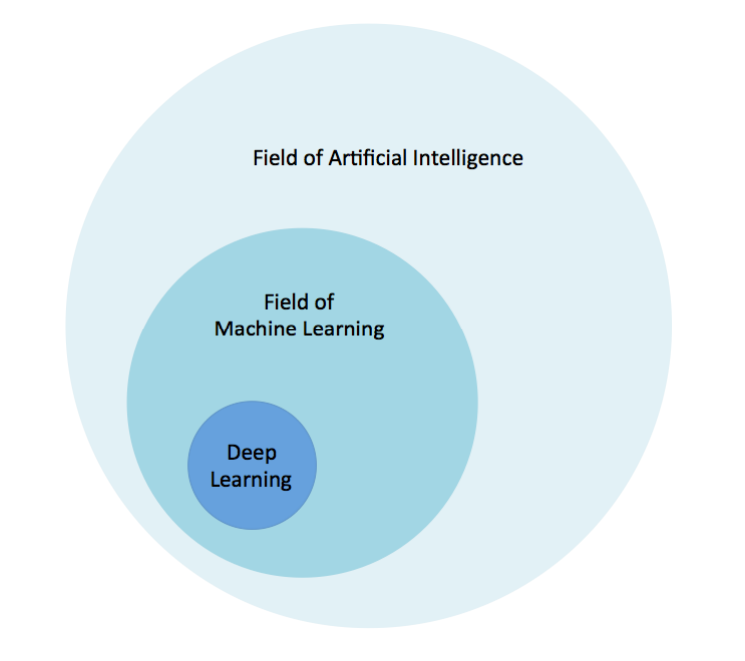
\includegraphics[width= 10cm]{../figuras/ia_ml.png}
  \caption{Relação entre inteligência artificial, aprendizado de máquina e aprendizado profundo \cite{dl-oreilly}}
  \label{fig:ia_ml}
\end{figure}

\section{Problema}

As tarefas de \textit{machine learning} são descritas de acordo com o processamento 
que o modelo deve realizar a partir de um exemplo de entrada (\textit{input}), em geral, descrito com 
um vetor $x \in \mathbb{R}^n, x=\{x_1, x_2, ..., x_n\}$.
Conforme explica \cite{Goodfellow-et-al-2016}, nas tarefas de classificação, o modelo deve prever a qual das $k$ categorias 
disponíveis um \textit{input} pertence, o algoritmo, então, cria uma função  
$ f : \mathbb{R}^n \rightarrow \{1,...,k\}$,  quando 
$ f(x) = y$, o vetor de entrada $x$ foi classificado na categoria $y$. Um exemplo 
de tarefa de classificação, no contexto deste trabalho, seria determinar se o 
consumo de cimento em um estado em um mês específico 
representa um aumento, queda ou estabilidade em relação ao mês anterior, essa 
análise, contudo, foge do escopo do estudo.

Outra categoria de tarefas são as de regressão, cujo objetivo é prever um valor numérico
a partir da entrada, a função criada pelo modelo, então, pode ser dada 
por $ f : \mathbb{R}^n \rightarrow \mathbb{R}$. 
Logo, o problema abordado neste trabalho pertence à categoria de regressão, 
uma vez que o objetivo é prever o valor do consumo de 
cimento em um estado e mês específicos a partir dos dados de entrada.

Ainda segundo \cite{Goodfellow-et-al-2016}, os problemas de aprendizado de máquina também podem ser divididos entre
 aprendizado não-supervisionado e supervisionado. No primeiro, o modelo recebe
um conjunto de dados (\textit{dataset}) não rotulado e então aprende
 propriedades da estrutura do \textit{dataset} e então
performa tarefas como a clusterização, que consiste em dividir o conjunto de dados
em \textit{clusters} com exemplos similares. No último, por sua vez, os dados de 
entrada estão associados a rótulos, resultados conhecidos, chamados de \textit{labels} ou
\textit{target} em inglês. Neste trabalho, a utiliza-se aprendizado supervisionado, uma vez 
que o obejtivo é utilizar os dados disponíveis para prever o consumo de cimento mensal
nos estados, um valor conhecido.

  
\section{Regressão linear}
\label{sec:reg_lin}

A regressão linear é um modelo de aprendizado de máquina que assume um relacionamento
linear entre a variável que será prevista (\textit{target}) e os dados de entrada.
Dessa forma, o objetivo é obter uma função linear que receba um vetor 
$x \in \mathbb{R}^n , x=\{x_1, x_2, ..., x_n\}$
como entrada e devolva a previsão de um escalar $y \in \mathbb{R}$. \cite{Goodfellow-et-al-2016}
Seja $\hat{y}$ o valor previsto pelo modelo para $\hat{y}$, então:

\begin{equation}
  \label{eq:reg_lin}
  \hat{y} = w^T x + b
\end{equation}

aonde $ w \in \mathbb{R}^n, w=\{w_1, w_2, ..., w_n\}$ é um vetor de parâmetros. Em 
particular, $w$ corresponde a um conjunto de pesos que 
determina como cada variável afeta a previsão. Então, se $x_i$
for associado a um peso $w_i$ positivo, aumentar o valor de $x_i$
resulta em um aumento na previsão $\hat{y}$, se $w_i$ for negativo, 
por outro lado, um aumento de $x_i$ resulta em diminuição de 
$\hat{y}$. Se $w_i$ for igual a 0, por sua vez, a 
variável $x_i$ não influencia no valor previsto.

A constante $b$, do inglês \textit{bias}, é um parâmetro para
mensurar viés, já que o \textit{output} da função é $b$ na ausência
de uma entrada. Dessa forma, a equação \ref{eq:reg_lin} pode ser escrita da 
seguinte forma: 

\begin{equation}
  \hat{y} = w_1 x_1 + w_2 x_2 + ... + w_n x_n + b
\end{equation}

Na ilustração abaixo, um exemplo de um modelo de regressão 
linear com apenas uma variável:

\begin{figure}[H] 
  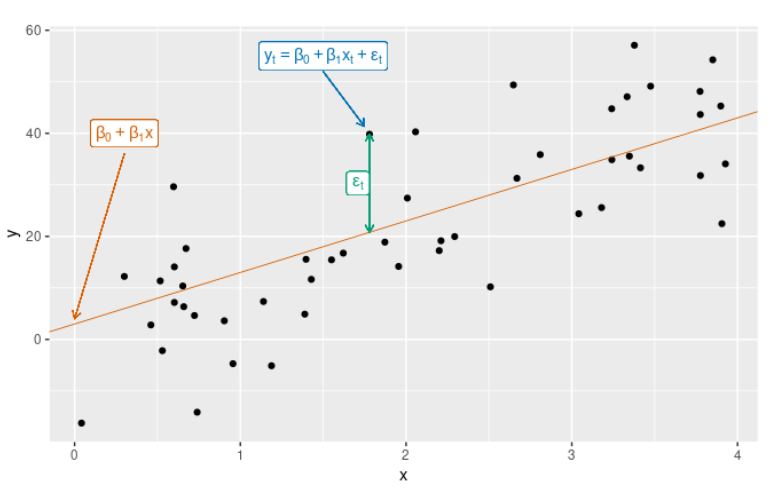
\includegraphics[width= 10cm]{../figuras/reg_lin.png}
  \caption{Exemplo de um modelo simples de regressão linear
  \cite{forecasting}}
  \label{fig:reg_lin}
\end{figure}

Nessa imagem, as observações estão 
representadas nos pontos pretos, enquanto a linha em laranja
corresponde à previsão realizada pelo modelo. Observa-se que
o modelo não prevê com total exatidão os dados observados, há 
um erro associado a cada previsão, como o destacado em verde 
na ilustração.

Dessa forma, cada observação $y_i$ possui um erro ${\varepsilon}_i$ 
associado e pode ser descrita por $y_i = w^T x_i + b + {\varepsilon}_i$.
O vetor de pesos $w$, então, é escolhido de modo a minimizar 
os erros em cada previsão.

Por se tratar de um modelo mais simples, é utilizada neste trabalho como base 
para comparar o desempenho de outros modelos mais robustos.

\section{Redes neurais}

Redes neurais são modelos computacionais inspirados no funcionamento
do cérebro animal, onde neurônios trabalham em paralelo sem 
uma unidade central de controle. Um neurônio biológico é uma célula 
nervosa que se comunica com outros neurônios e passa impulsos 
eletro-químicos de uma célula para outra por meio das sinapses.
A comunicação entre neurônios, sinapse, ocorre apenas se o impulso 
for forte o bastante para ativar a liberação de
químicos na fenda sináptica.

Um neurônio é composto de vários dendritos, um axônio e corpo 
celular, como na imagem \ref{fig:neuron}. 

\begin{figure}[H] 
  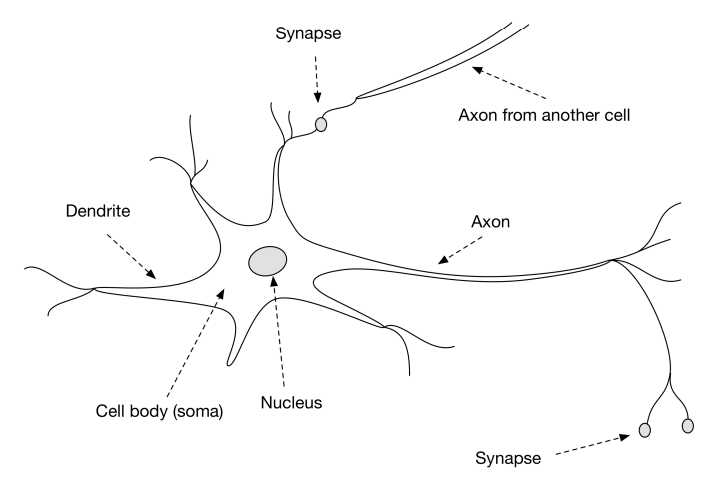
\includegraphics[width= 12cm]{../figuras/neuron.png}
  \caption{Ilustração de um neurônio biológico. \cite{dl-oreilly}
  Destaca-se a informação chegando a um dendrito do neurônio
  por meio de uma sinapse, além de uma sinapse que se inicia no axônio 
  do neurônio e propaga informação a diante.
  }
  \label{fig:neuron}
\end{figure}

Os dendritos recebem 
informações de outros neurônios vizionhos, na forma de impulsos
elétricos, e conduzi-las até o corpo celular. Ao chegar no corpo
celular, a informação é processada e novos impulsos são gerados. 
Essa informação é, então, repassada para outro neurônio 
através do axônio por meio de sinapse. Dessa forma, sinapse é o
ponto de contato entre a terminação axônica de um neurônio e o 
dendrito de outro.\cite{deeplearningbook}. 

A estrutura e funcionamento dos neurônios biológicos foram 
base para os cientistas criarem neurônios artificiais, como 
os \textit{perceptrons}. 

\subsection{Neurônios artificiais}

O \textit{perceptron}, foi desenvolvido em 1957 por Frank 
Rosenblatt, inspirado nos trabalhos de Warren McCulloch e Walter Pitts.
Trata-se de um modelo linear de classificação binária que 
recebe $n$ entradas e produz uma saída binária, como mostrado 
na ilustração simplificada \ref{fig:perceptron-simples}.\cite{deeplearningbook}
Esse modelo inicial apresentava limitações e foi evoluído com o passar do 
tempo, as redes neurais atualmente, em geral, utilizam 
outro modelo de neurônio como ilustrado em \ref{fig:perceptron}.


\begin{figure}[H] 
  \centering
  \begin{subfigure}{7cm}
    \centering 
    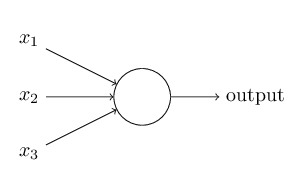
\includegraphics[width=7cm]{../figuras/perceptron-simples.png}
    \caption{Visão simplificada de um neurônio \cite{deeplearningbook}}
    \label{fig:perceptron-simples}
  \end{subfigure}
  \hfill
  \begin{subfigure}{7cm}
    \centering
    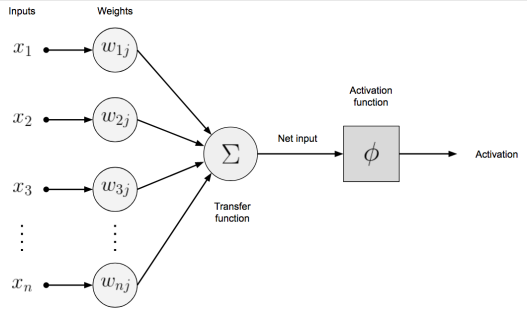
\includegraphics[width=7cm]{../figuras/perceptron.png}
    \caption{Ilustração da arquitetura de um 
    neurônio artificial \cite{dl-oreilly}}
    \label{fig:perceptron}
  \end{subfigure}
\end{figure}

Como é possível observar na figura \ref{fig:perceptron}, cada
uma das entradas $x_i$ está associada a um peso $w_i$. Os pesos
$w_1, w_2, ..., w_n$ expressam a importância das respectivas
entradas para o valor de saída, de modo semelhante à 
regressão linear na seção \ref{sec:reg_lin}. O produto escalar entre
os pesos e as respectivas entradas, chamada de \textit{net input}
na imagem \ref{fig:perceptron}, passa por uma função de 
ativação $\phi$ que determina a saída do neurônio. 
Além disso, um valor de \textit{bias} ou polarização é
adicionado ao produto escalar para aumentar a liberdade 
da função. O \textit{bias} possibilita que 
um neurônio que possua todas as entradas nulas a 
apresente saída não nula, dessa forma,
aumenta a capacidade de aproximação da rede. 
\cite{deeplearningbook}


Seja $x$ o vetor das $n$ entradas do neurônio, então
$x \in \mathbb{R}^n, x=\{x_1, x_2, ..., x_n\}$, seja também 
$w$ o vetor com os pesos associados a cada entrada, 
$w \in \mathbb{R}^n, w=\{w_1, w_2, ..., w_n\}$. Além disso,
seja $b$ o valor de \textit{bias} e $\Phi$ a função de ativação.
Dessa forma, o \textit{output} de um neurônio é dado por:
 
\begin{equation}
  h_{w,b} = \Phi(w \cdot x + b)
\end{equation}

Essa saída é utilizada como uma das entradas dos neurônios
na camada seguinte, de modo a formar a estrutura das redes 
neurais semelhante ao funcionamento do cérebro. Os neurônios,
então, formam a unidade que compõe as redes neurais artificiais,
como ilustrado na figura abaixo:

\begin{figure}[H] 
  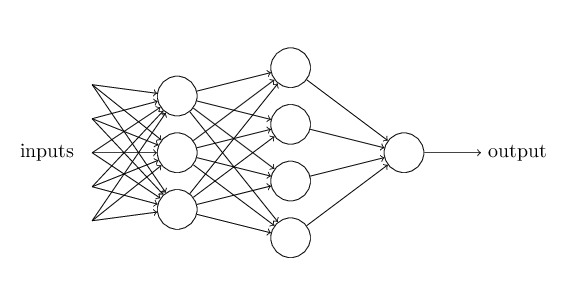
\includegraphics[width= 12cm]{../figuras/rede-neural.png}
  \caption{Ilustração de uma rede neural simples.\cite{deeplearningbook}}
  \label{fig:redeneural}
\end{figure}


\subsection{Função de ativação}

A função de ativação propaga a saída de um 
neurônio na rede neural para a camada seguinte. Enquanto os pesos 
e o \textit{bias} realizam uma transformação linear nos dados 
de entrada, a função de ativação aplica uma transformação não
linear e dessa forma torna possível que a rede neural resolva
problemas não lineares e complexos, como reconhecer padrões de 
escrita.\cite{deeplearningbook}

A função de ativação é um atributo de cada uma das camadas 
da rede e é escolhida de acordo com a tarefa que será 
executada, por exemplo, a função sigmóide é recomendada
 para problemas de classificação. Neste trabalho, 
foram utilizada: \textit{rectified linear unit} (ReLU) e \textit{swish}.

\subsubsection{Rectified linear unit (ReLU)}

A função ReLU, do inglês \textit{rectified linear unit}, é o 
estado da arte atualmente, uma vez que apresenta bom desempenho 
em diferentes tarefas. \cite{dl-oreilly} A função ReLu é dada por:

\begin{equation}
  f(x) = max(0,x)
\end{equation}

Ao utilizar essa função, a derivada, utilizada para atualizar
os pesos e \textit{bias} no treinamento da rede, é zero, quando 
a entrada é nula ou uma constante, como na imagem abaixo. Dessa
forma, a ReLU não sofre do problema da dissipação do gradiente como
a sigmóide.

\begin{figure}[H] 
  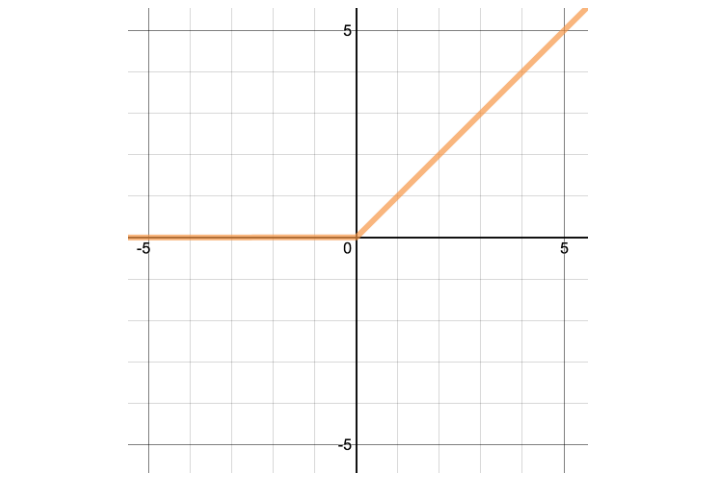
\includegraphics[width= 8cm]{../figuras/relu.png}
  \caption{Rectified linear unit (ReLU) \cite{dl-oreilly}}
  \label{fig:relu}
\end{figure}

\subsubsection{Swish}

A função \textit{swish} foi proposta por pesquisadores da 
Google com a prerrogativa de apresentar melhor desempenho 
que a ReLU em redes neurais profundas. \cite{swish}

A \textit{swish} é uma função não monotônica e suave 
dada por:

\begin{equation}
  f(x) = x \cdot sigmoid(x) = \frac{x}{1+e^{-x}}
\end{equation}


O gráfico da função é similar ao da ReLU:

\begin{figure}[H] 
  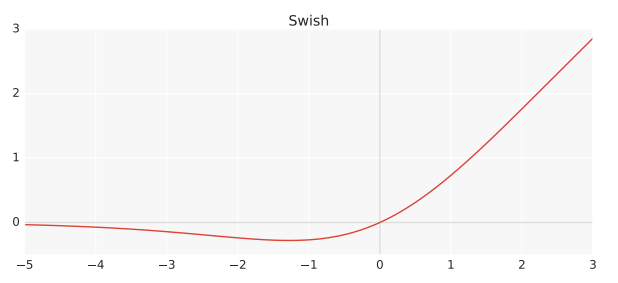
\includegraphics[width= 8cm]{../figuras/swish.png}
  \caption{Função \textit{swish} \cite{swish}}
  \label{fig:swish}
\end{figure}

\subsection{Redes neurais multi-layer perceptrons}
  % dar uma melhorada -> parte do com o treinamento fornecido
  % se agredar -> combinação -> melhorar
  % redes de arquitetura multilayer ...
  % o "e feedforward" não tem nada a ver -> é um passo do treinamento  -> sequencia dos dados de entrada
Redes neurais são modelos de \textit{machine learning} 
inspiradas no cérebro humano aonde o aprendizado ocorre 
ao se agregarem neurônios matemáticos que 
estabelecem conexões de acordo com o treinamento fornecido. 
Neste trabalho, aplicaram-se redes 
\textit{multilayer perceptrons} (MLPs), ou seja, que 
apresentam múltiplas camadas de neurônios 
e \textit{feedfoward}, onde a saída de 
uma camada de neurônios é utilizada como entrada para a camada seguinte, sem utilizar retropropagação.
          
        
\subsection{Redes Neurais Recorrentes}
\label{rnn}

Se por um lado as redes neurais tradicionais são projetadas
para realizar previsões sem modelar dimensão temporal, as redes
neurais recorrentes se diferem por capturar informação de contexto, ou seja,
histórico, para realizar previsões. Essa dimensão temporal, então, se dá por 
meio de ciclos nas conexões, ou \textit{feedback loops}, como mostrado na 
figura abaixo.


\begin{figure}[H]
  \centering
  \begin{subfigure}{7cm}
      \centering
      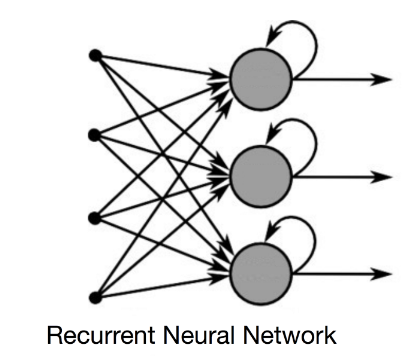
\includegraphics[width=7cm]{../figuras/redes/rnn.png}
      \caption{Redes neurais recorrentes}
  \end{subfigure}
  \hfill
  \begin{subfigure}{7cm}
      \centering
      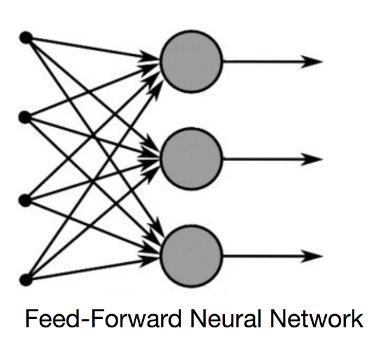
\includegraphics[width=7cm]{../figuras/redes/ff.png}
      \caption{Redes \textit{feed forward}}
  \end{subfigure}
\end{figure}

Dessa forma, os neurônios nas redes recorrentes recebem entradas de ativação 
de seu próprio estado atual e dos nós anteriores na rede, não apenas dos anteriores
na rede, como nas redes tradicionais.

As redes recorrentes, então, não recebem como entrada apenas um vetor de tamanho 
fixo como as redes \textit{feed forward}, seu \textit{input} é formado 
por vários vetores, um para cada \textit{time-step}. Na figura abaixo, o número
total de amostras corresponde ao campo "examples", o vetor com as 
variávies de entrada ao campo "inputs" ou "values per time step" (na 
figura de Recurrent Network Data) e o tamanho das sequências consideradas
pelo modelo ao "time steps". 

\begin{figure}[H] 
  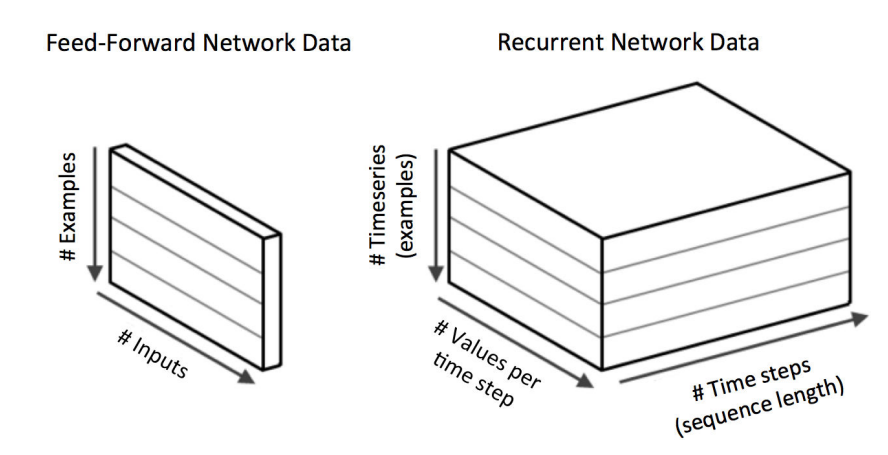
\includegraphics[width= 12cm]{../figuras/redes/input-rnn.png}
  \caption{Comparação entre a entrada de uma rede neural tradicional
  e um recorrente \cite{dl-oreilly}}
  \label{fig:input-rnn}
\end{figure}

Redes recorrentes são uma subclasse das redes neurais, contudo, possuem mais
de uma categoria, neste trabalho testaram-se as redes LSTM e GRU.

\subsubsection{LSTM}

As redes Long Short Term Memory (LSTM) foram introduzidas em 1997 por Hochreiter 
and Schmidhuber\footnote{\cite{lstm-origem}} e são a variação mais utilizada das redes
neurais recorrentes atualmente, por exemplo para classificar séries temporais, 
reconhecimento de fala e de escrita a mão. Redes LSTM apresentam células de 
memória conectadas, o conteúdo dessas células é modulado pelo \textit{input gate} e o \textit{forget gate},
por exemplo, se ambos estiverem fechados em um tempo o conteúdo da célula permanecerá 
o mesmo no tempo em questão e no próximo. Essa estrutura permite que a informação
seja retida ao longo do tempo e evita o problema do \textit{vanishing gradient} que 
ocorre com a maioria das redes recorrentes.

As redes neurais LSTM apresentam uma arquitetura diferente 
das redes tradicionais, uma vez que há ciclos de \textit{feedback}
nas conexões entre as células. Para melhor ilustrar essa 
arquitetura, \cite{dl-oreilly} utiliza a visualização \textit{flat} 
ou achatada das redes neurais, na qual as células de uma mesma 
camada da rede estão representadas como um único nó.
Pode-se observar essa representação em \label{fig:comparacao-ff-flat-normal},
na imagem \ref{fig:arq-ff} está a representação tradicional 
de uma rede neural \textit{feed forward}, já em em 
\ref{fig:arq-ff-flat} está a mesma rede com a represetnação 
achatada.

\begin{figure}[H]
  \centering
  \begin{subfigure}{7.5cm}
      \centering
      \label{fig:arq-ff}
      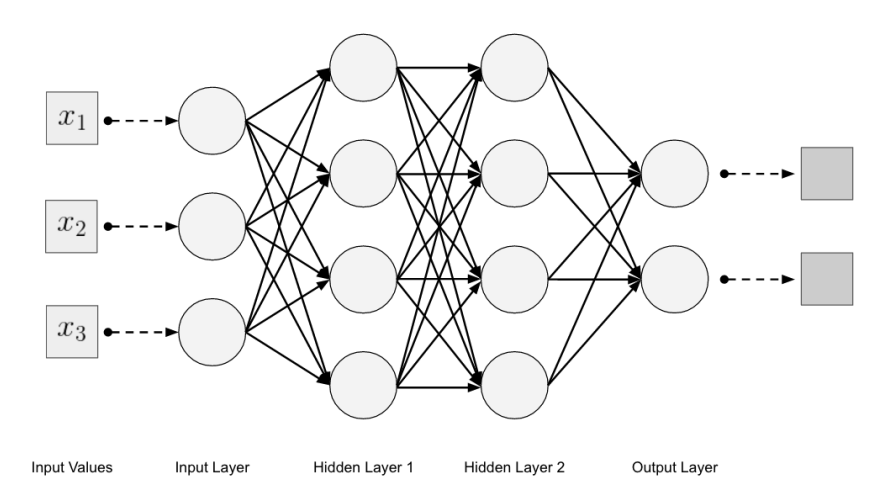
\includegraphics[width=7.5cm]{../figuras/redes/arq-ff.png}
      \caption{Arquitetura de rede neural \textit{feed forward}}
  \end{subfigure}
  \hfill
  \begin{subfigure}{7.5cm}
      \centering
      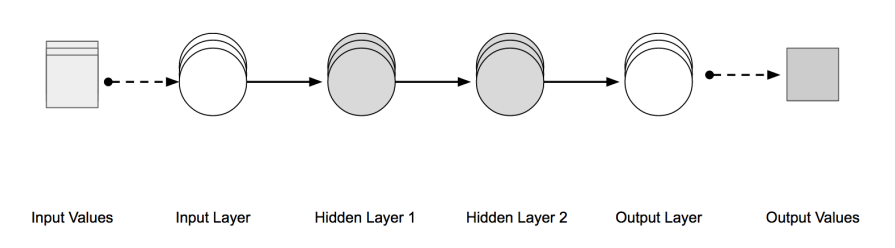
\includegraphics[width=7.5cm]{../figuras/redes/arq-ff-flat.png}
      \caption{Visão \textit{flat} (achatada) arquitetura de rede neural \textit{feed forward} }
      \label{fig:arq-ff-flat}
  \end{subfigure}
  \label{fig:comparacao-ff-flat-normal}
\end{figure}

As redes LSTM introduzem o conceito de conexão entre a saída de uma das 
camadas ocultas da rede neural com a entrada da mesma camada. A partir desse
ciclo, obtém-se entradas de tempos anteriores como parte da informação que 
chega à rede neural no tempo atual. Na figura \ref{fig:arq-rnn-flat}, essas 
conexões recorrentes são representadas como as setas que saem de uma célula e 
atingem a mesma célula, uma vez que utiliza-se a representação achatada.
A imagem \ref{fig:arq-rnnff}, por sua vez, representa a rede LSTM desenrolada 
atráves do eixo do tempo.

\begin{figure}[H]
  \centering
  \begin{subfigure}{7.5cm}
      \centering
      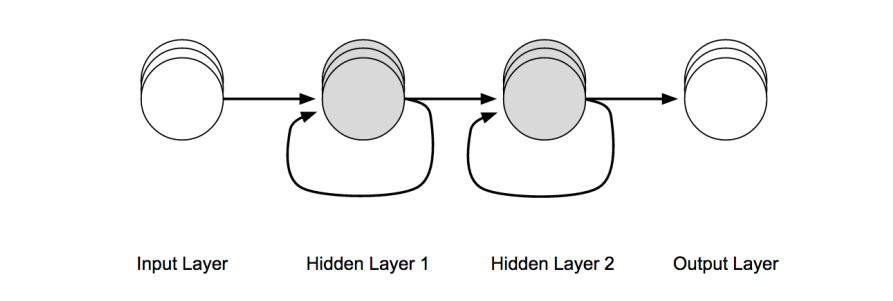
\includegraphics[width=7.5cm]{../figuras/redes/arq-rnn-flat.png}
      \caption{Visão \textit{flat} (achatada) arquitetura de rede neural LSTM }
      \label{fig:arq-rnn-flat}
  \end{subfigure}
  \begin{subfigure}{7.5cm}
    \centering
    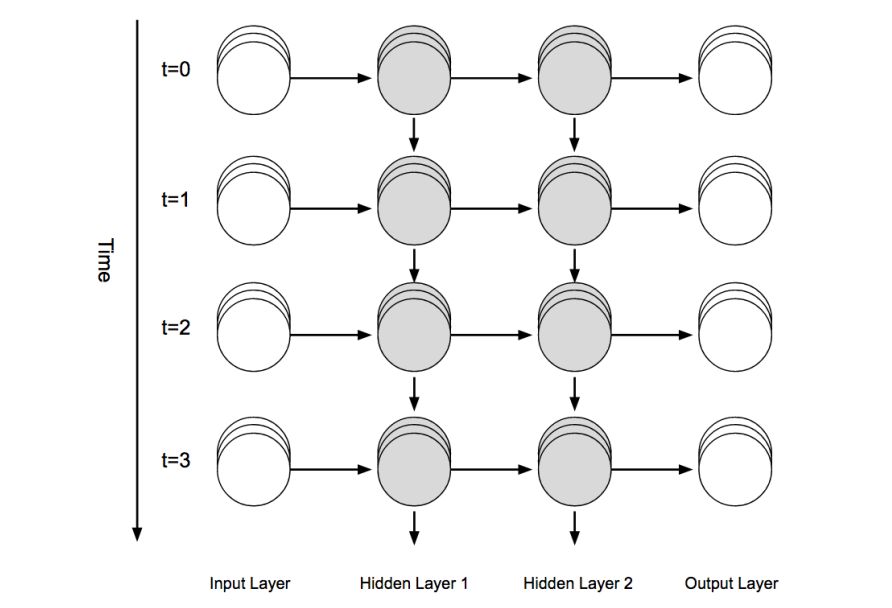
\includegraphics[width=7.5cm]{../figuras/redes/arq-rnn.png}
    \caption{Visão da rede neural LSTM ao longo do tempo}
    \label{fig:arq-rnnff}
  \end{subfigure}
  \hfill
  \label{fig:comparacao-rnn-flat-normal}
\end{figure}

As unidades que formam cada uma das camadas de uma LSTM são uma variação dos
neurônios artificiais clássicos. Essas unidades, representadas em \ref{fig:lstm-cell},
 permitem que a rede mantenha o estado
ao longo tempo e apresentam dois tipos de 
conexões: conexões vindas da camada anteriores e vindas \textit{outputs} dessa
mesma unidade em tempos anteriores.

\begin{figure}[H]
  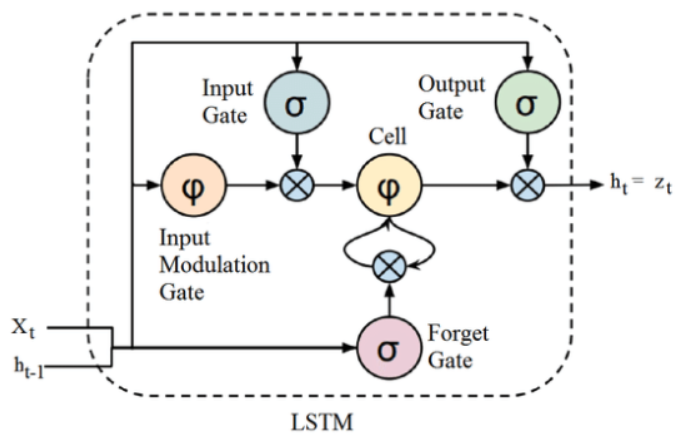
\includegraphics[width=9cm]{../figuras/redes/lstm-cell.png}
  \caption{Célula de memória de rede LSTM \cite{deeplearningbook}}
  \label{fig:lstm-cell}
\end{figure}

A unidade LSTM recebe duas entradas, a observação no tempo atual e a saída do 
último estado oculto. Nas unidades LSTM, a informação é retida nas células e as manipulações de memória 
são realizadas nos \textit{gates} (portões). O \textit{forget gate} é responsável
por remover informações que não são mais úteis para a célula, ou seja, pelo 
esquecimento, essa operação é realizada por meio de multiplicação de matrizes 
de pesos, adição de parâmetro de viés e função de ativação que fornece uma saída binária. 
O \textit{input gate}, por sua vez, adiciona informações úteis ao estado da célula
a partir da aplicação de funções sigmoides e tangente hiperbólica, além da multiplicação de vetores. 
Já o \textit{output gate} extrai informações úteis ao estado da célula atual 
para apresentar como saída da célula e entrada para a próxima com funções tangente
hiperbólica e sigmoide, além da multiplicação de vetores. \cite{deeplearningbook}

\subsubsection{GRU}

As GRU, sigla para \textit{gated recurrent units} no inglês,
são unidades recorrentes similares às LSTM. Enquanto as unidades
das redes LSTM apresentam dois estados passados entre as células, 
estado da célula e estado oculto, que carregam memória, respectivamente,
de longo e curto prazo, as unidades GRU apresentam apenas um 
estado oculto carregado ao longo do tempo e capaz de manter
as dependências de curto e longo prazo ao mesmo tempo. A 
estrutura das unidades GRU pode ser vista em \ref{fig:gru-cell}.

\begin{figure}[H]
  \centering
  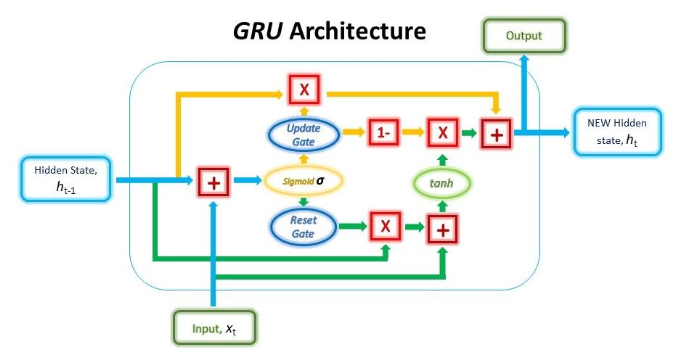
\includegraphics[width=9cm]{../figuras/redes/gru-cell.png}
  \caption{Unidade da rede GRU \cite{deeplearningbook}}
  \label{fig:gru-cell}
\end{figure}

As unidades GRU apresentam portões, assim como as unidades LSTM,
para controlar o fluxo de informações. O \textit{reset gate}, ou
portão de redefinição, é responsável por controlar quais informações 
das etapas anteriores serão mantidas com as da etapa atual por meio 
da função sigmoide e multiplicação de vetores. O \textit{update gate},
por sua vez, tem como objetivo determinal quanto das informações
armazenadas no estado oculto anterior devem ser retidas para 
o futuro.


\subsection{Normalização}

O objetivo da normalização dos dados, é garantior que as variáveis de entrada 
estejam na mesma escala. Esse processo é necessário não apenas para realizar melhor comparação entre variáveis 
com diferentes unidades, mas também para o melhor funcionamentos dos algoritmos 
de aprendizado, uma vez que se as \textit{features} estiverem em escalas diferentes
os pesos podem ser atualizados mais rápidos que outros.

\subsubsection{\textit{Standard scaler}}

O \textit{standard scaler} garante que as variáveis de entrada estejam em uma 
escala com as propriedades de uma distribuição normal, ou seja, média ($\mu$)
igual a zero e variância ($\sigma$) igual a um. Dessa forma, a operação 
realizada para aplicar o processo em um entrada $x$ é

\begin{equation}
  z = \frac{x - \mu}{\sigma}
\end{equation}

\subsubsection{\textit{Min-Max scaler}}

O \textit{min-max scaler} transforma os dados de modo que a 
escala dos dados tenha um itnervalo definido, em geral, entre
0 e 1.

\begin{equation}
  X_{norm} = \frac{X - X_{min}}{X_{max} - X_{min}}
\end{equation}